% Figure 1: Microtubule Lattice Geometry
% Shows cross-section (13 protofilaments) and longitudinal view with helical lattice
\documentclass[tikz,border=5pt]{standalone}
\usepackage{tikz}
\usetikzlibrary{calc,patterns,decorations.pathmorphing,positioning}

\begin{document}
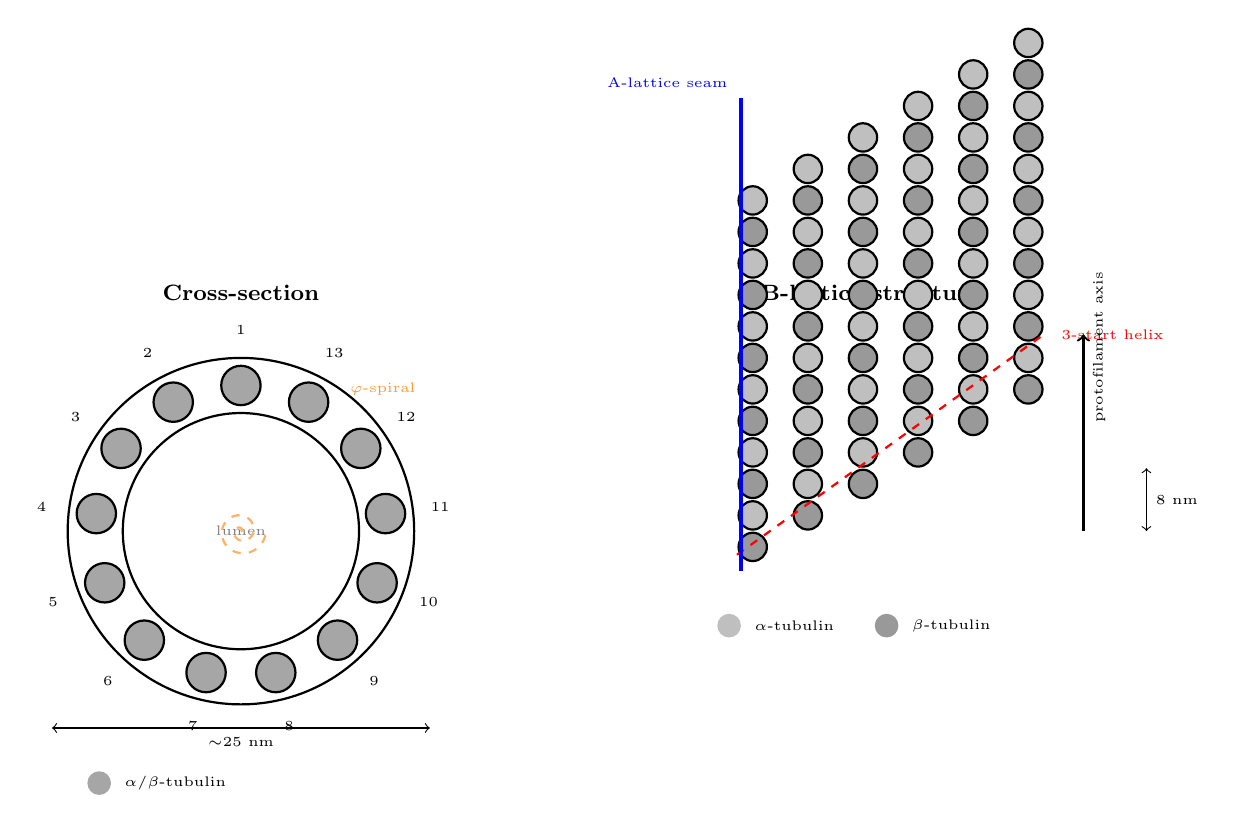
\begin{tikzpicture}[scale=1]

% === LEFT PANEL: Cross-section view ===
\begin{scope}[shift={(-4,0)}]
    % Title
    \node[above,font=\footnotesize\bfseries] at (0,2.8) {Cross-section};

    % Outer circle (microtubule wall)
    \draw[thick] (0,0) circle (2.2);
    \draw[thick] (0,0) circle (1.5);

    % 13 protofilaments as circles around the ring
    \foreach \i in {1,...,13} {
        \pgfmathsetmacro{\angle}{90 + (\i-1)*360/13}
        \pgfmathsetmacro{\rad}{1.85}
        % Alpha tubulin (darker)
        \fill[gray!70] (\angle:\rad) circle (0.25);
        \draw[thick] (\angle:\rad) circle (0.25);
        % Protofilament number
        \node[font=\tiny] at (\angle:2.55) {\i};
    }

    % Inner lumen
    \node[font=\tiny,gray] at (0,0) {lumen};

    % Diameter annotation
    \draw[<->,thin] (-2.4,-2.5) -- (2.4,-2.5);
    \node[below,font=\tiny] at (0,-2.5) {$\sim$25 nm};

    % Legend
    \fill[gray!70] (-1.8,-3.2) circle (0.15);
    \node[right,font=\tiny] at (-1.6,-3.2) {$\alpha/\beta$-tubulin};
\end{scope}

% === RIGHT PANEL: Longitudinal/unrolled lattice view ===
\begin{scope}[shift={(2.5,0)}]
    % Title
    \node[above,font=\footnotesize\bfseries] at (1.5,2.8) {B-lattice structure};

    % Draw tubulin dimer grid (helical lattice pattern)
    % 6 columns (protofilaments) x 6 rows
    \foreach \col in {0,...,5} {
        \foreach \row in {0,...,5} {
            % Offset every other column for helical pattern
            \pgfmathsetmacro{\yoff}{\col*0.4}
            \pgfmathsetmacro{\xpos}{\col*0.7}
            \pgfmathsetmacro{\ypos}{\row*0.8 + \yoff}

            % Alpha tubulin (top of dimer)
            \fill[gray!50] (\xpos,\ypos+0.2) circle (0.18);
            \draw[thick] (\xpos,\ypos+0.2) circle (0.18);

            % Beta tubulin (bottom of dimer)
            \fill[gray!80] (\xpos,\ypos-0.2) circle (0.18);
            \draw[thick] (\xpos,\ypos-0.2) circle (0.18);
        }
    }

    % Helical line showing 3-start helix
    \draw[red,thick,dashed] (-0.2,-0.3) -- (3.7,2.5);
    \node[red,font=\tiny,right] at (3.8,2.5) {3-start helix};

    % Protofilament direction arrow
    \draw[->,thick] (4.2,0) -- (4.2,2.5);
    \node[right,font=\tiny,rotate=90] at (4.4,1.25) {protofilament axis};

    % Seam indicator
    \draw[blue,very thick] (-0.15,-0.5) -- (-0.15,5.5);
    \node[blue,font=\tiny,left] at (-0.2,5.7) {A-lattice seam};

    % Dimer spacing
    \draw[<->,thin] (5,0) -- (5,0.8);
    \node[right,font=\tiny] at (5,0.4) {8 nm};

    % Legend
    \fill[gray!50] (-0.3,-1.2) circle (0.15);
    \node[right,font=\tiny] at (-0.1,-1.2) {$\alpha$-tubulin};
    \fill[gray!80] (1.7,-1.2) circle (0.15);
    \node[right,font=\tiny] at (1.9,-1.2) {$\beta$-tubulin};
\end{scope}

% === Golden ratio spiral overlay (subtle) ===
\begin{scope}[shift={(-4,0)}]
    \draw[orange!60,thick,dashed,domain=0:720,samples=200,smooth]
        plot ({0.08*\x/180*cos(\x)},{0.08*\x/180*sin(\x)});
    \node[orange!80,font=\tiny] at (1.8,1.8) {$\varphi$-spiral};
\end{scope}

\end{tikzpicture}
\end{document}
